\input{preamble}

\usepackage{comment}

\begin{document}

% ----------------------------------------------------------------
\begin{titlepage}

\center % Center everything on the page

\fancypagestyle{firststyle}
{
\cfoot{Москва, 2021}
\renewcommand{\headrulewidth}{0pt}
}

\thispagestyle{firststyle}


%----------------------------------------------------------------------------------------
%	LOGO SECTION
%----------------------------------------------------------------------------------------

 \includegraphics[width=0.4\textwidth]{./pics/msu_logo}\\[0.2cm] % Include a department/university logo - this will require the graphicx package

%----------------------------------------------------------------------------------------
%	HEADING SECTIONS
%----------------------------------------------------------------------------------------

\textsc{\small Московский государственный университет имени М.В.Ломоносова}\\ % Name of your university/college
\textsc{\small Факультет вычислительной математики и кибернетики}\\ % Major heading such as course name
\textsc{\small  }\\[3cm] % Minor heading such as course title

%----------------------------------------------------------------------------------------
%	TITLE SECTION
%----------------------------------------------------------------------------------------
{
	Бабаков Вадим Валерьевич
} \\[1cm]
{ \Large \bfseries
	Разработка метода подавления линейного размытия на изображениях с помощью свёрточных нейронных сетей
} \\[1cm]
{ \Large
	Курсовая работа
}\\[2.5cm] % Title of your document
 
%----------------------------------------------------------------------------------------
%	AUTHOR SECTION
%----------------------------------------------------------------------------------------

\vfill
\begin{flushright}
\large 
\textbf{Научный руководитель:}\\
Старший научный сотрудник, к.ф.-м.н.\\
Насонов Андрей Владимирович
\end{flushright}
 
%----------------------------------------------------------------------------------------

\vfill % Fill the rest of the page with whitespace

\end{titlepage}% ----------------------------------------------------------------


\tableofcontents

\newpage

\pagestyle{fancy}

\rhead{\thepage}
\fancyfoot{}

\section{Введение}
Линейное размытие -- тип ухудшения качества изображения, возникающий при съёмке камерой из-за долгой экспозиции.
% Восстановление размытого изображения – одна из важных задач в области компьютерного зрения.
\par
На фотографии, сделанной с мобильного устройства, зачастую размытие возникает даже при короткой выдержке. В этом случае оно хорошо аппроксимируется линейным размытием. То есть линейно размытое изображение можно рассматривать как свёртку изначального неразмытого изображения и ядра размытия. Для применения большинства алгоритмов восстановления изображения необходимо точно определить неизвестное ядро размытия, и от этой точности сильно зависит качество их работы.
\par
В связи с широким распространением мобильных устройств с наличием камеры и ростом разрешения сенсора возникает задача восстановления резкости для снимков, сделанных с короткой выдержкой. Это обусловлено следующим фактом: при большой выдержке ядро размытия может иметь сложную форму, искать его сложнее, но при небольшой можно предполагать, что движение постоянное, и его направление не меняется, то есть размытие линейное. В этом случае ядро размытия у такого изображение можно представить как комбинацию ядра линейного размытия и расфокусировки. 
% Использование этой модели позволяет снизить вычислительную сложность алгоритма. 
% В данной работе будут рассматриваться изображения, размытые в результате движения самой камеры, то есть параметры размытия объектов на изображении, находящихся на примерно одинаковом расстоянии от камеры, будут также примерно одинаковы.


\subsection{Существующие методы восстановления изображения от размытия}
Есть много алгоритмов определения размытия вслепую (только по изначальному изображению). Например, методы, работающие в пространственной области: их основная идея заключается в том, чтобы восстанавливать ядро размытия по локальным характеристикам изображения (точки, линии, края) \cite{kopeika, chalmond, Wu}. В описанных методах тип размытия должен быть известен заранее, перед вычислением ядра. 
В дополнение вычисление будет неточным при сильном размытии, потому что становится сложно выделять характеристики изображения. 

Также существуют методы, работающие в частотной области \cite{rom, cannon}, которые основаны на том, что частотный отклик у ядер содержит пересечение с нулём с некоторым периодом. В \cite{lokh} описан метод для выделения направления и длины размытия. Главный недостаток этих алгоритмов заключается в том, что они крайне чувствительны к зашумлению \cite{kundur}.
\par
Актуальные методы, основанные на глубоком обучении (использовании нейронных сетей) показали своё превосходство в задачах обращения линейного размытия. Многие работы до них использовали подход, основанный на различных способах регуляризации либо заменой некоторых операций предобученными сетями \cite{shuler, sun}. В современных методах зачастую создают полноценную нейронную сеть, на вход получающую размытое изображение, результатом работы которой является восстановленное изображение \cite{nah, tao}. 

\newpage
\section{Постановка задачи}
В работе ставится задача повышения качества размытых изображений, полученных при съёмке с небольшой выдержкой, путём использования свёрточных нейронных сетей.

Предполагается, что параметры ядра размытия не являются постоянными для всего изображения, в этом случае стандартные методы определения его параметров не работают. В данной работе предлагается находить ядро размытия изображения в спектральной области. 
\par
% с помощь какого мтеода нужно искать решение
%  1) хотим искать ядро ращмытия в спектральной области
%  2) приводим ядра
%  3) на преобрвазлоянивах фурье видно, что линейное размытие приводит к частотным повторениям в амлитуде
% 4) оьращаем внимание на одномерное преобразование фурье
%  5) линейно размытие -длинный прямоугольник
%  6) пример прямоугольника в случае прямоугольного одномиерного сигнала
%  7) ооснование, почему считаетсчя логарифм, а не просто модуль
%  8) если без него, то вклад дальних гармоник очень мал
%  9) бдет легче найти периодичность
% 10) 

\begin{figure}[h!]
  \centering
  \begin{subfigure}[b]{0.4\linewidth}
    \includegraphics[width=\linewidth]{pics/linear_motion_blur/bicycle.jpg}
    %  \caption{Coffee.}
  \end{subfigure}
  \begin{subfigure}[b]{0.4\linewidth}
    \includegraphics[width=\linewidth]{pics/linear_motion_blur/traffic.jpg}
    % \caption{More coffee.}
  \end{subfigure}
  \begin{subfigure}[b]{0.5\linewidth}
    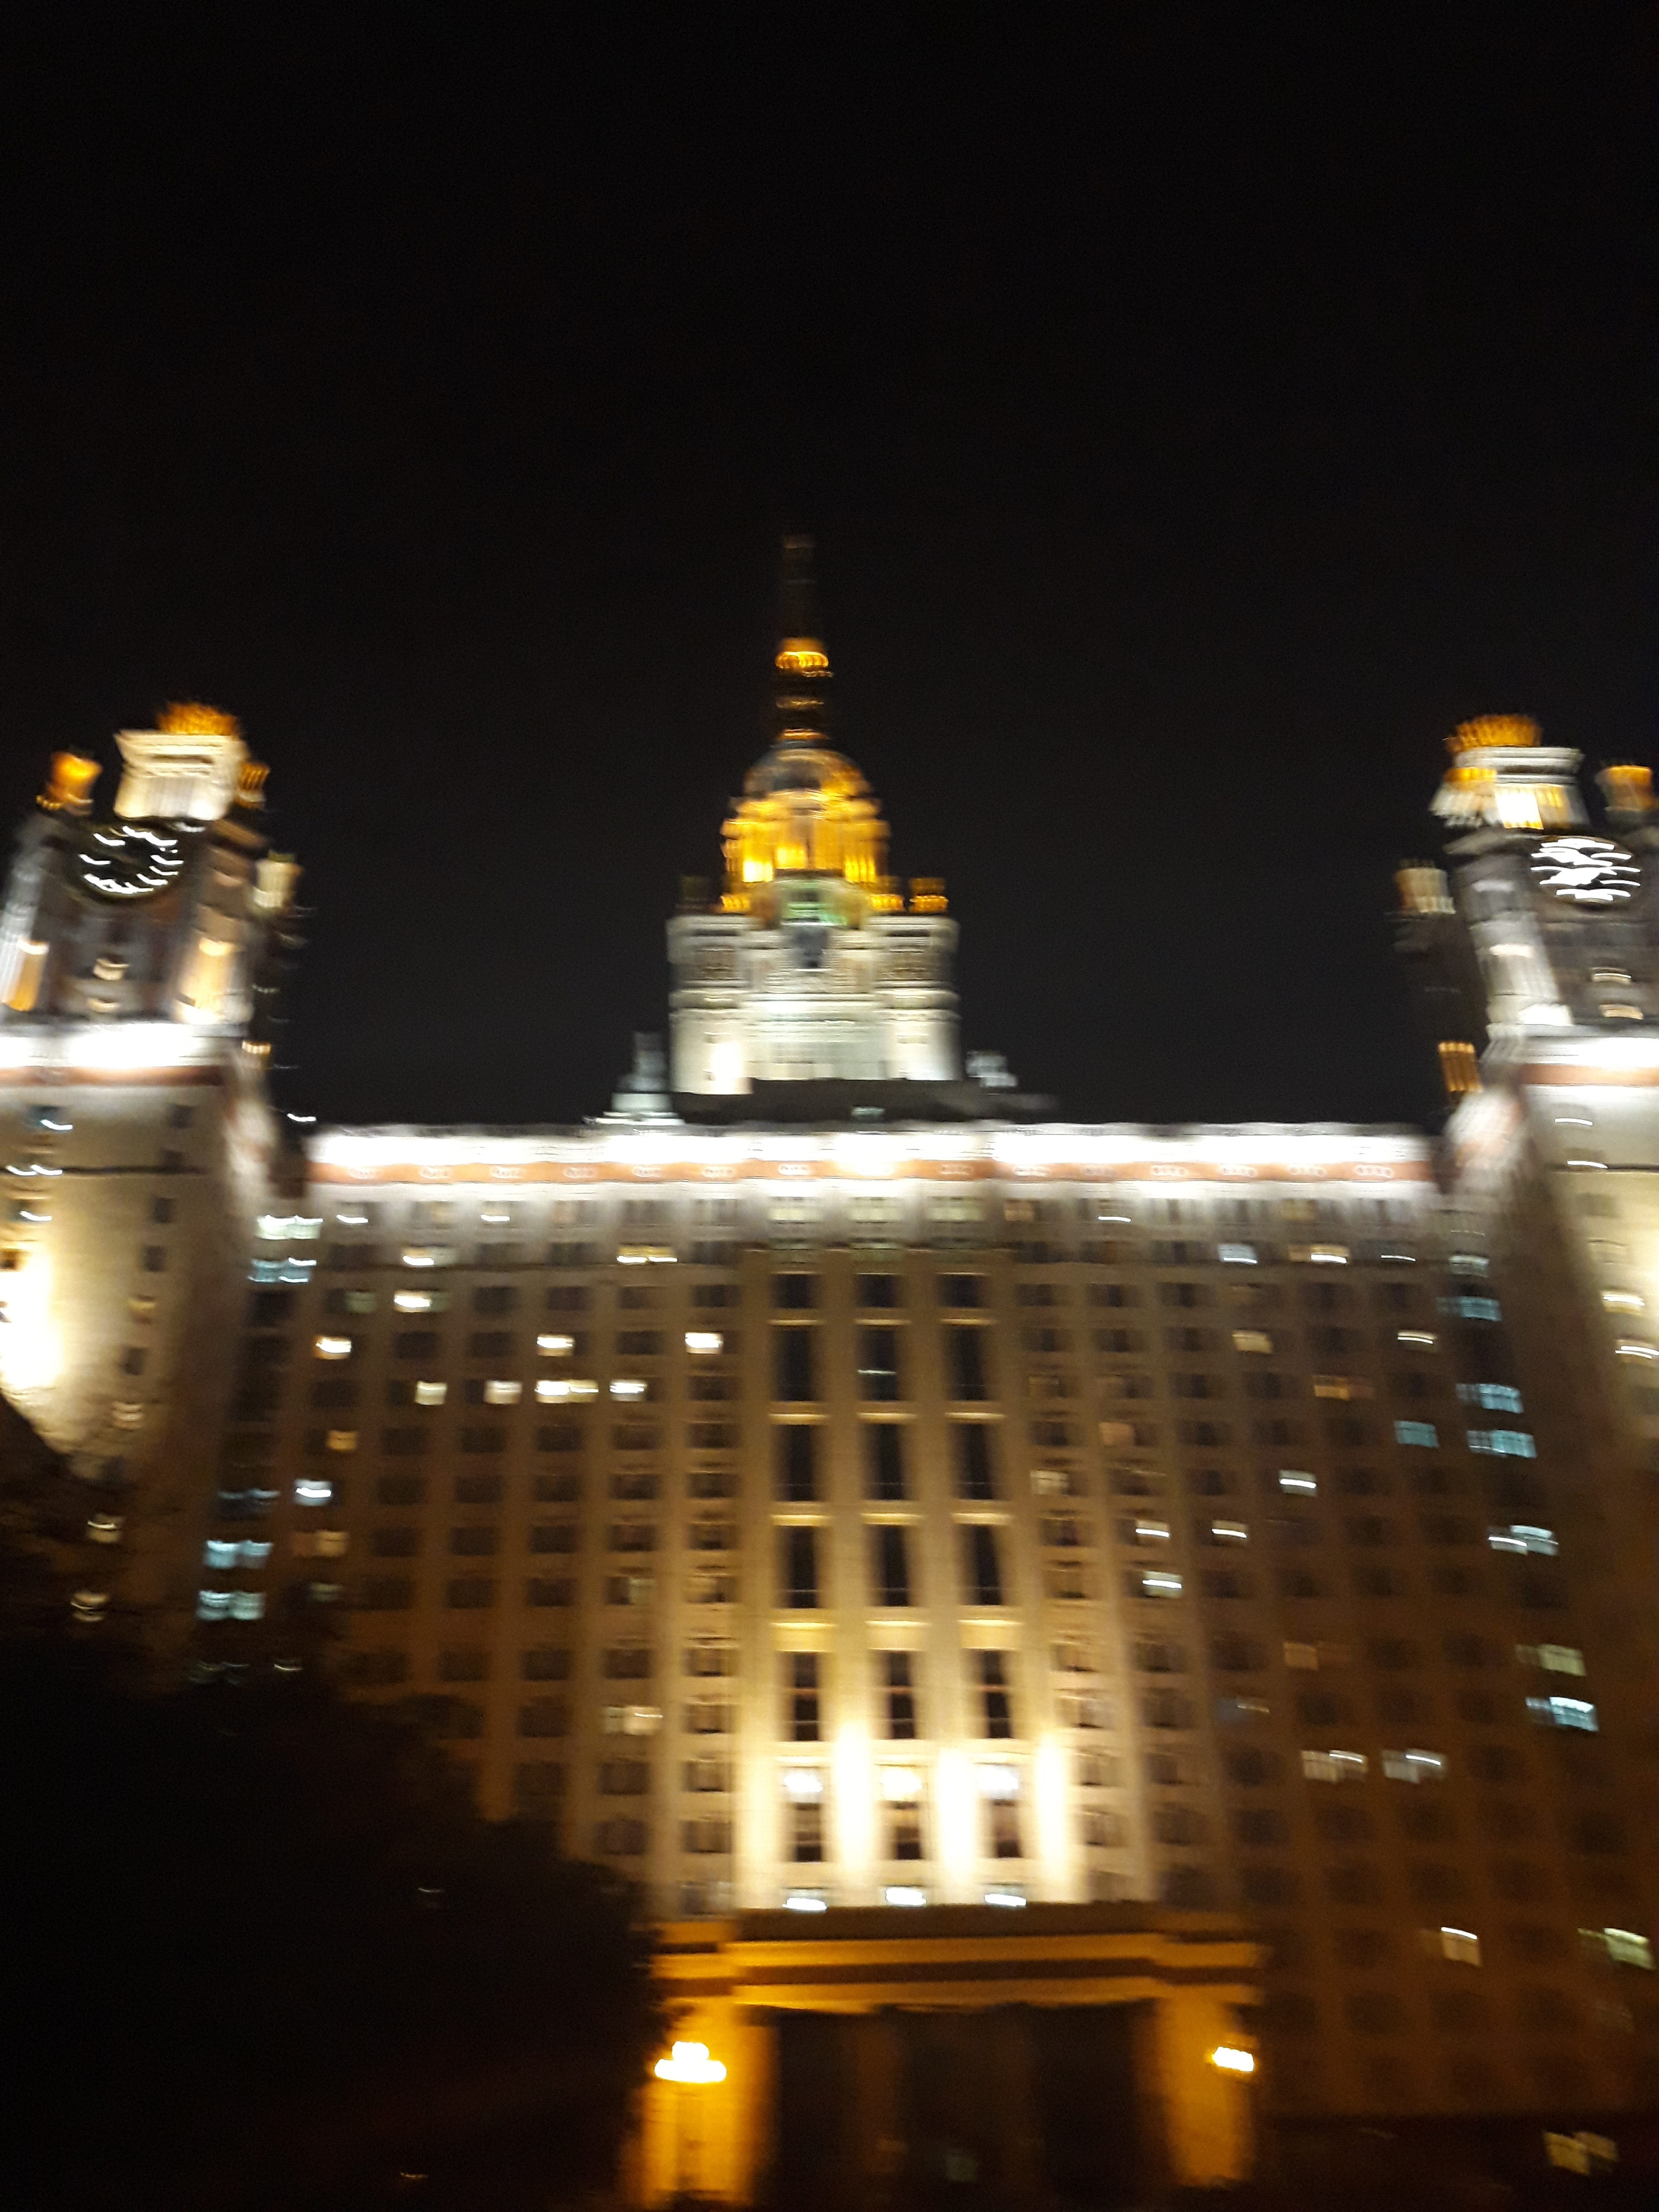
\includegraphics[width=\linewidth]{pics/linear_motion_blur/mb0.jpg}
    % \caption{Too much coffee.}
  \end{subfigure}
  \caption{Примеры неравномерного линейного размытия на изображениях}
  \label{fig:lblur}
\end{figure}

\subsection{Цель работы}
Разработать и программно реализовать метод восстановления линейно размытого изображения, основанный на использовании свёрточных нейронных сетей и опирающийся на стандартные методы при определении параметров размытия на изображении.


\subsection{Используемая математическая модель }
Предполагая, что размытие постоянное для всего изображения, 
размытое изображение можно выразить в следующем виде:
\begin{equation}
g(x, y)=f(x, y) \otimes d(x, y)+n(x, y),
\label{conv_formula}
\end{equation}
где $f(x,y)$ - изначальное изображение, $d(x, y)$ - ядро размытия, $n(x,y)$ - добавочный шум, а знак $\otimes$ обозначает свёртку $$(f * d)(x, y)=\int_{-\infty}^{+\infty} \int_{-\infty}^{+\infty} f\left(\tau_{1}, \tau_{2}\right) \cdot d\left(x-\tau_{1}, y-\tau_{2}\right) d \tau_{1} d \tau_{2}$$
В работе \cite{kopeika} продемонстрировано, что такая модель даёт возможность достаточно точно выразить различные типа размытия на практике. 
Например, для размытия типа дефокуса ядро может быть представлено как функция:
\begin{equation}
d(x, y)=\left\{\begin{array}{ll}
0 & \sqrt{x^{2}+y^{2}}>R \\
1 /\left(\pi R^{2}\right) & \sqrt{x^{2}+y^{2}} \leq R
\end{array}\right.
\end{equation}
где радиус размытия $R$ прямо пропорционален силе размытия. 
Ядро размытия в движении выражается как прямоугольная функция:
\begin{equation}
d(x, y)=\left\{\begin{array}{ll}
 1/L & y = \alpha x, \sqrt{x^{2}+y^{2}} \leq L/2 \\
0 & \text { иначе}
\end{array}\right.
\end{equation}
где  $\alpha$  - угол направления движения относительно оси $x$, 
а $L$ - длина размытия.
\par
Так как размытое изображение является результатом свёртки с ядром, в пространственной области выделение размытия является невозможным. Однако, параметры размытия можно определить, используя кепструм.

Кепструм $C_{g}(p, q)$ изображения $g(x,y)$ определяется следующим образом:
\begin{equation}C_{g}(p, q)=F^{-1}\{\ln |F(g)|\}
\label{cepstrum_def}
\end{equation}
где  $F(g) = \frac{1}{\sqrt{2 \pi}} \int\limits_{-\infty}^{+\infty} \int\limits_{-\infty}^{+\infty} g(x, y) e^{-2 \pi i (x u+v y)} d x d y$  - двумерное преобразование Фурье функции $g(x,y)$.
% ,
%  $g(x,y) = F^{-1}{G(u,v)} = \frac{1}{\sqrt{2 \pi}} \int\limits_{-\infty}^{+\infty} \int\limits_{-\infty}^{+\infty} G(u,v) e^{(2 \pi(x u+v y)} d x d y$  - обратное преобразование Фурье.



 Преобразование Фурье ядра линейного размытия формализуется следующим образом:
\begin{equation}
D(u, v)=\frac{\sin (\pi L w)}{\pi L w}, \text{ где } w = x cos(\alpha) + y sin(\alpha)
\label{motion_blur_fourier}
\end{equation}
\par

Наглядно демонстрируется (Рис. \ref{ris:sinc}), что $D(u,v)$ - функция $sinc$ с нулями, возникающими в точках $w=\pm \frac{1}{L}, \pm \frac{2}{L}, \cdots$
Также важно отметить, что для корректности вычислений (из-за того, что функция $ln(x)$ 
при $x$, близких к нулю, стремится к~$-\infinity$) есть смысл считать кепструм следующим образом:
$$C_{g}(p, q)=F^{-1}\{\ln 1+ |G(u, v)|\}$$
На рисунке \ref{ris:sinc} можно увидеть, что линейное размытие приводит к определённым закономерностям в амплитуде в частотной области преобразования Фурье изображения.
\par

\begin{figure}[H]
\begin{minipage}[h]{0.4\linewidth}
\center{\includegraphics[width=1\linewidth]{pics/ceps/lena.png}} а)\\ 
\end{minipage}
    \hfill
\begin{minipage}[h]{0.4\linewidth}
\center{\includegraphics[width=1\linewidth]{pics/ceps/lena_Ceps.png}} б)\\ 
\end{minipage}
    \vfill
\begin{minipage}[h]{0.4\linewidth}
\center{\includegraphics[width=1\linewidth]{pics/ceps/lena_blurred.png}} в)\\ 
\end{minipage}
    \hfill
\begin{minipage}[h]{0.4\linewidth}
\center{\includegraphics[width=1\linewidth]{pics/ceps/sinc_ceps.png}} г)\\
\end{minipage}

\caption{Спектры изображений: (а) изначальное изображение, (б) спектр изначального изображения, (в) размытое под углом в 45 градусов изображение, (г) спектр размытого изображения}
\label{ris:sinc}
\end{figure}

Рассматриваемый в работе тип размытия, размытие в движении, возникает при движении устройства, фиксирующего изображение(камера здесь и далее), относительно снимаемой сцены. 
Для упрощения модели предполагается, что камера двигается с постоянной скорость в одном и том же направлении. Метод, предлагаемый в данной работе, позволяет определять параметры размытия (для линейного - длина и направление), используя преобразование Радона \cite{oliv}.

% На преобразованиях Фурье видно, что линейное размытие приводит к определённым закономерностям в амплитуде в частотной области. 

\newpage
\section{Предлагаемый метод}

В данной работе предлагается сократить размерность рассматриваемых параметров линейного размытия при восстановлении до одного - длины размытия. Сделать это предлагается по следующему алгоритму:
\begin{enumerate} 
    \item Определить угол размытия на изображении
    \item Повернуть изображение таким образом, чтобы определённое на предыдущем шаге направление размытия совпало с горизонталью
    \item Восстановить изображение совокупностью предобучнных нейронных сетей 
    \item Повернуть изображение обратно на угол, определённый на первом шаге
\end{enumerate}


\subsection{Определение угла размытия}

Как описано выше, зачастую размытие на изображении неравномерное, и кепстр всего изображения не даёт возможности определить параметры размытия. Для решения этого предлагается разбивать изображения на блоки меньшего размера и считать параметры отдельно в каждом из блоков независимо друг от друга.
Предполагается, что в пределах одного блока размытие постоянное.

В работе для определения угла размытия на изображении предлагается использовать преобразование Радона.

Определение преобразования Радона вещественной функции $\phi(x, y)$,
определённой в $\mathbb{R}^{2}$, с углом $\theta$ на расстоянии $\rho$:
$$
\mathcal{R}(\phi, \rho, \theta)=\int\limits_{-\infty}^{\infty} \int\limits_{-\infty}^{\infty} \phi(x, y) 
\delta(\rho-x \cos \theta-y \sin \theta) d x d y
$$
где $\delta$ - дельта-функция Дирака. Запись выше эквивалентна следующему:
$$
\mathcal{R}(\phi, \rho, \theta)=\int\limits_{-\infty}^{\infty} 
\phi(\rho \cos \theta-s \sin \theta, \rho \sin \theta+s \cos \theta) d s
$$
Преобразование Радона $\mathcal{R}(\phi, \rho, \theta)$ 
эквивалентно интегралу функции $\phi$ вдоль прямой, составляющей угол $\theta$
с осью $x$ и расположенной на расстоянии $\rho$ от точки начала координат. 

%  Ядро размытия везде своё, но оно меняется постепенно
%  Предполагается, что ядро размытия в одном блоке постоянно, находим его для блоков
%  Дальше берём модель из статьи
% Будут блоки, где размытие нельзя будет определить - привести пример
% Иделаьные патич для анализа - те, где нет 
% Набор патчиков с найденным направлением
\par

Использовать преобразование Радона для вычисления угла размытия было предложено в \cite{moghaddam}. 
Там же в качестве угла, отвечающего углу размытия, используется значение, отвечающее максимуму преобразования Радона. 

\begin{figure}[H]
\begin{minipage}[h]{0.32\linewidth}
\center{\includegraphics[width=1\linewidth]{pics/sinogram/square.png}}
\end{minipage}
\hfill
\begin{minipage}[h]{0.32\linewidth}
\center{\includegraphics[width=1\linewidth]{pics/sinogram/local_cepstrum.png}}
\end{minipage}
\hfill
\begin{minipage}[h]{0.32\linewidth}
\center{\includegraphics[width=1\linewidth]{pics/sinogram/sin.PNG}}
\end{minipage}
\begin{minipage}[h]{1\linewidth}
\begin{tabular}{p{0.32\linewidth}p{0.32\linewidth}p{0.32\linewidth}}
\centering а) & \centering б) & \centering в) \\
\end{tabular}
\end{minipage}
\vspace*{-1cm}
\caption{Процесс определния угла размытия: а) Фрагмент изображения, б) Кепструм фрагмента, в) Синограмма кепструма.}
\label{ris:correlationsignals}
\end{figure}

\subsubsection{Параметрическая модель}
При вычислении параметров размытия можно столкнуться со следующей проблемой: 
изображения содержат области, из которых нельзя получить информацию о размытии, 
то есть объекты однородной структуры без выделяющихся элементов, например, 
чистое небо или ровная стена (\ref{ris:bad_ceps}). Также необходимо учитывать, что определение параметров 
размытия по части изображения может давать ложную информацию (например, в областях с ярковыраженным  краем, не сонаправленным размытию)

Таким образом, для корректности восстановления изображения необходимо построить параметрическую модель, 
которая будет учитывать неправильно определённые параметры размытия, с учётом того, что размытие на изображении
меняется от блока к блоку постепенно.

Так как предполагается, что на рассматриваемом изображении размытие постоянное,
можно взять в качестве параметров размытия некое среднее значение соответствующих параметров
(длина и угол направления размытия). Предлагаемый вариант: использовать медианное значение по каждому из параметров.  

\begin{figure}[H]
\begin{minipage}[h]{0.4\linewidth}
\center{\includegraphics[width=1\linewidth]{pics/bad_ceps/sky.PNG}} \\ 
\end{minipage}
\hfill
\begin{minipage}[h]{0.4\linewidth}
\center{\includegraphics[width=1\linewidth]{pics/synth_blur/i1.png}} \\ 
\end{minipage}
    \vfill
\begin{minipage}[h]{0.4\linewidth}
\center{\includegraphics[width=1\linewidth]{pics/bad_ceps/sky1.PNG}} \\ 
\end{minipage}
\hfill
\begin{minipage}[h]{0.4\linewidth}
\center{\includegraphics[width=1\linewidth]{pics/synth_blur/i2.png}} \\
\end{minipage}

\caption{Пример областей изображения, по которым нельзя сделать вывод о параметрах размытия. Справа - соответствующие им кепстры (цвета инвертированы)}
\label{ris:bad_ceps}
\end{figure}

По итогу для каждого изображения получаем соответствующее ему число - предполагаемый угол размытия. Важно отметить, что метод работает не со 100\%-точностью (пример гистограммы распределния ошибки можно увидеть на рисунке \ref{ris:angle_histogram}). Но это в данной работе не критично, об этом подробнее в следующем пункте.

\begin{figure}[H]
\center{\includegraphics[width=1\linewidth]{pics/hist.png}} \\ 
\caption{Гистограмма ошибок определения угла вышеописанным алгоритмом}
\label{ris:angle_histogram}
\end{figure}

\newpage
\subsection{Восстановление изображения}
Для восстановления предлагается использовать совокупность нейронных сетей, каждая из которых дообучена на изображениях, зашумлённых и искусственно размытых ядрами размытия с фиксированным углом (0 градусов)
и различающимися длинами (3, 5, 7, 9 и 11 пикселей).

Таким образом, получается последовательность нейронных сетей, каждая из которых "специализируется" на своей длине размытия, но при этом (в силу того, что перед дообучением берётся не чистая нейронная сеть, а уже предобученная на восстановление от линейного размытия) достаточно хорошо восстанавливает в целом любые изображения, деградированные линейным размытием. 

\subsubsection{Выбор модели нейронной сети}
 (?) Здесь нужен анализ актуальных методов восстановления линейного размытия?
Или достаточно описать, мол, из трёх актуальных рассматриваемых моделей быстрее и лучше дообучалась выбранная? И насколько подробно вдаваться в архитектуру выбранной нейронной сети?

Deep Multi-scale Convolutional Neural Network for Dynamic Scene Deblurring
DeblurGAN-v2
Neural Blind Deconvolution Using Deep Priors 

\subsubsection{Устойчивость метода при неправильно определённых параметрах размытия}

Необходимо отметить, что предлагаемый метод более устойчив к некорректному определению параметров размытия, чем стандартные. Для примера сравним с итеративным методом обращения свёртки, основанный на использовании функционала полной вариации. 

\begin{figure}[H]
\begin{minipage}[8]{1\linewidth}
\center{\includegraphics[width=1\linewidth]{pics/plots/PSNR_a.png}} 
\\ 
\end{minipage}
    \vfill
\begin{minipage}[8]{1\linewidth}
\center{\includegraphics[width=1\linewidth]{pics/plots/SSIM_a.png}} 
\\
\end{minipage}
%     \vfill
% \begin{minipage}[t]{0.45\linewidth}
% \center{\includegraphics[width=1\linewidth]{pics/plots/PSNR_l.png}} 
% \\ 
% \end{minipage}
% \hfill
% \begin{minipage}[t]{0.45\linewidth}
% \center{\includegraphics[width=1\linewidth]{pics/plots/SSIM_l.png}} 
% \\
% \end{minipage}
\caption{ Графики качества восстановления изображений при различной ошибки определения угла направления размытия алгоритмом }
\label{ris:plots_a}
\end{figure}

По метрикам качества изображений в случае ошибки определения угла (Рис. \ref{ris:plots_a}) лучше себя показывает метод обращения свёртки, но при его использовании возникают серьёзные графические артефакты (рингинг), чего не происходит при применении предлагаемого метода \ref{ris:Wrong_angle}

\begin{figure}[H]
\begin{minipage}[t]{0.3\linewidth}
\center{\includegraphics[width=1\linewidth]{pics/restore_ex/b_img_19.png}} 
(a) Размытое изображение\\ 
\end{minipage}
\hfill
\begin{minipage}[t]{0.3\linewidth}
\center{\includegraphics[width=1\linewidth]{pics/error_angle/dec_img_19.png}} 
(б) Восстановленное обращением свёртки\\ 
\end{minipage}
\hfill
\begin{minipage}[t]{0.3\linewidth}
\center{\includegraphics[width=1\linewidth]{pics/error_angle/nn_img_19.png}} 
(в) Результат работы предложенного алгоритма\\ 
\end{minipage}
\caption{ Пример работы сравниваемых алгоритмов в случае большой ошибки в предполагаемом угле направления размытия (40 градусов) }
\label{ris:Wrong_angle}
\end{figure}


\begin{figure}[H]
\begin{minipage}[t]{1\linewidth}
\center{\includegraphics[width=1\linewidth]{pics/plots/PSNR_l.png}} 
\\ 
\end{minipage}
\begin{minipage}[t]{1\linewidth}
\center{\includegraphics[width=1\linewidth]{pics/plots/SSIM_l.png}} 
\\
\end{minipage}
\caption{ Графики качества восстановления изображений при различной ошибке определения длины размытия алгоритмом }
\label{ris:plots_l}
\end{figure}


\begin{figure}[H]
\begin{minipage}[t]{0.3\linewidth}
\center{\includegraphics[width=1\linewidth]{pics/restore_ex/b_img_19.png}} 
(a) Размытое изображение\\ 
\end{minipage}
\hfill
\begin{minipage}[t]{0.3\linewidth}
\center{\includegraphics[width=1\linewidth]{pics/restore_ex/dec_img_19.png}} 
(б) Восстановленное обращением свёртки\\ 
\end{minipage}
\hfill
\begin{minipage}[t]{0.3\linewidth}
\center{\includegraphics[width=1\linewidth]{pics/restore_ex/nn_img_19.png}} 
(в) Результат работы предложенного алгоритма\\ 
\end{minipage}


\caption{ Сравнение итеративного подхода к обращению свёртки и предложенного метода в случае отсутствия ошибки при определении параметров размытия. Важно отметить, что итеративный подход затратен по времени, в отличие от использования нейронной сети, и требует в среднем на 2 порядка больше времени}
\label{ris:restore_comparison}
\end{figure}

\newpage
\section{Результаты работы алгоритма}

\begin{figure}[H]
% \begin{minipage}[t]{0.4\linewidth}
% \center{\includegraphics[width=1\linewidth]{pics/restore_ex/b_img_12.png}} 
% \\ 
% \end{minipage}
% \hfill
% \begin{minipage}[t]{0.4\linewidth}
% \center{\includegraphics[width=1\linewidth]{pics/restore_ex/nn_img_12.png}} 
% \\ 
% \end{minipage}
%     \vfill
\begin{minipage}[t]{0.45\linewidth}
\center{\includegraphics[width=1\linewidth]{pics/restore_ex/b_img_14.png}} 
\\ 
\end{minipage}
\hfill
\begin{minipage}[t]{0.45\linewidth}
\center{\includegraphics[width=1\linewidth]{pics/restore_ex/nn_img_14.png}} 
\\
\end{minipage}
    \vfill
\begin{minipage}[t]{0.45\linewidth}
\center{\includegraphics[width=1\linewidth]{pics/restore_ex/b_img_17.png}} 
\\ 
\end{minipage}
\hfill
\begin{minipage}[t]{0.45\linewidth}
\center{\includegraphics[width=1\linewidth]{pics/restore_ex/nimg_17.png}} 
\\
\end{minipage}


\caption{ Примеры результата работы алгоритма. Слева - размытые зашумлённые изображения, справа - восстановленные }
\label{ris:restore_example}
\end{figure}



\begin{figure}[H]
\begin{minipage}[t]{0.22\linewidth}
\center{\includegraphics[width=1\linewidth]{pics/restore_ex/01.png}} 
(a) Размытое изображение\\ 
\end{minipage}
\hfill
\begin{minipage}[t]{0.22\linewidth}
\center{\includegraphics[width=1\linewidth]{pics/restore_ex/02_whyte.png}} 
(б) Whyte и др.\\ 
\end{minipage}
\hfill
\begin{minipage}[t]{0.22\linewidth}
\center{\includegraphics[width=1\linewidth]{pics/restore_ex/03_krishnan.png}} 
(в) Krishnan и др.\\ 
\end{minipage}
\hfill
\begin{minipage}[t]{0.22\linewidth}
\center{\includegraphics[width=1\linewidth]{pics/restore_ex/04_sun.png}} 
(г) Sun и др.\\ 
\end{minipage}
    \vfill
\begin{minipage}[t]{0.22\linewidth}
\center{\includegraphics[width=1\linewidth]{pics/restore_ex/05_xu.png}} 
(д) Xu и др.\\ 
\end{minipage}
\hfill
\begin{minipage}[t]{0.22\linewidth}
\center{\includegraphics[width=1\linewidth]{pics/restore_ex/06_pan.png}} 
(е) Pan и др.\\
\end{minipage}
\hfill
\begin{minipage}[t]{0.22\linewidth}
\center{\includegraphics[width=1\linewidth]{pics/restore_ex/07_deepdeblur.png}} 
(ж) DeepDeblur\\
\end{minipage}
\hfill
\begin{minipage}[t]{0.22\linewidth}
\center{\includegraphics[width=1\linewidth]{pics/restore_ex/08_DeblurGANv2.png}} 
(з) Предложенный метод\\
\end{minipage}

\caption{Сравнение качества восстановления размытого изображения предложенным методом. Отмечу, что предложенный метод восстанавливает изображения без заметных визуальных артефактов}
\label{ris:restore_example_big}
\end{figure}

\newpage
\section{Заключение}
Был разработан подавления линейного размытия наизображениях с помощью свёрточных нейронных сетей и была создана программная реализация разработанного алгоритма.
В рамках данной работы программная реализация алгоритма была протестирована
на искусственно размытых изображениях и изображениях, ухудшенных естественным образом, и показала свою практическую применимость.


\newpage
\printbibliography[heading=bibintoc]

\end{document}